Typesetting documents faster comes down to becoming more familiar with VSCode and the use of snippets.
\section{Becoming familiar with VSCode}
It's worth taking a look at the official trips and tricks: \href{https://code.visualstudio.com/docs/getstarted/tips-and-tricks}{link}.
We will cover some of the simpler ones which are used constantly.
\subsection{Multi-line editing}
You can set your cursor in the same position across multiple lines using
\texttt{ctrl+alt+\keys{\arrowkeyup}/\keys{\arrowkeydown}} (on Mac \keys{\cmd + \Alt + \arrowkeyup}/\keys{\arrowkeydown}).

\begin{figure}[h]
\centering
    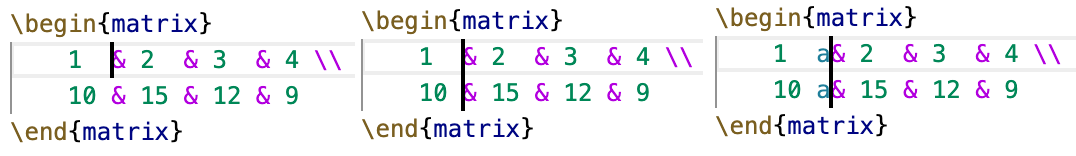
\includegraphics[width=0.7\textwidth]{figures/multiline.png}
\caption{Multiline editing}
\end{figure}

\subsection{Moving lines}
You can move the current line with \keys{\Alt + \arrowkeyup}/\keys{\arrowkeydown}.

The existence of this command is the motivation for why paragraphs are split at the end of each sentence, allowing you to easily reorganise your ideas.

\subsection{Copying lines}
You can copy the current line with \keys{\shift + \Alt + \arrowkeyup}/\keys{\arrowkeydown}.

This is particularly useful with maths and tables.

\subsection{Identing code}
Indent in: \keys{\ctrl + ]} (Mac \keys{\cmd + ]}).\\
Indent out: \keys{\ctrl + [} (Mac \keys{\cmd + [}).
\subsection{Command pallete}
\keys{\ctrl+\shift+P} (Mac: \keys{\cmd+\shift+P}) opens all the commands given by your extensions.
In particular, Math Preview Panel, View LaTeX PDF File, and Promote/Demote sections are used quite often.


\section{Using snippets}
The LaTeX Workshop extension provides many snippets, which can be seen \href{https://github.com/James-Yu/LaTeX-Workshop/wiki/Snippets}{here}.
They can also be user defined, and as you typeset more documents you will find your particular needs.
More information on writing your own snippets can be found \href{https://code.visualstudio.com/docs/editor/userdefinedsnippets}{here}.

A few examples will be presented, and we will go over the keybindings to very quickly produce them.
Bear in mind the pure text sections will just be ignored.

\paragraph{Note:}
In case you are unfamiliar with the symbols:
\begin{table}[h] \centering
\begin{tabular}{cc}
    Symbol & Meaning \\ \hline
    \keys{\Alt} &\texttt{alt}\\ 
    \keys{\shift} & \texttt{shift}\\
    \keys{\cmd} & \texttt{command}\\
    \keys{\tab} & \texttt{tab}
\end{tabular}
\end{table}

\subsection{Example - Logarithms}
This is a small section from the wikipedia article \href{https://en.wikipedia.org/wiki/Irrational_number#Logarithms}{Logarithms} which we recreate.
Highlighted below are only the snippets, so you would still have to manually write things like \verb|\log_2 3| for \( \log_2 3 \).

\begin{figure}[h]
\centering
    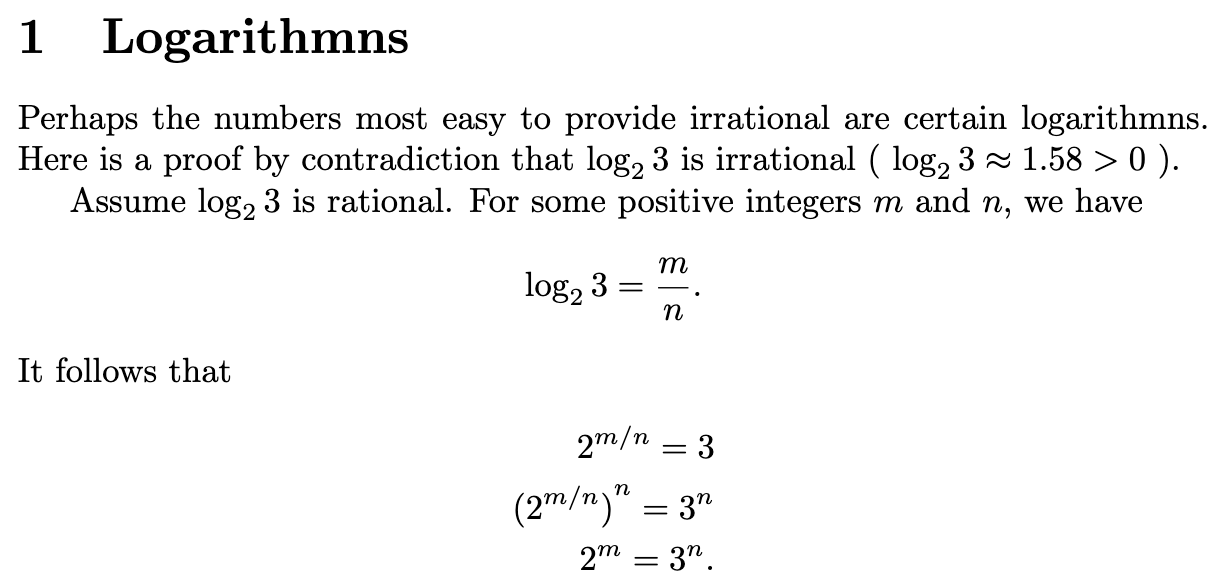
\includegraphics[width=0.6\textwidth]{figures/logarithmns.png}
\end{figure}

\begin{enumerate}
    \item \keys{sse + \tab} creates \verb|\section{}|. \keys{\tab} again after typing ``Logarithmns'' to move cursor out of the brackets.
    \item For the intext maths, the time saving is \keys{$\backslash$( + \tab}.
    \item \keys{bseq + \tab } quickly creates the unnumbered \texttt{equation*} environment
    \item \keys{@/ + \tab} to create the fraction. type \keys{m + \tab + n}
    \item For the next maths environment, we use \keys{bsal+\tab} --- creating an \texttt{align*} environment
    \item \keys{2 + ** + \tab + m/n + \tab} creates \( 2^{m/n} \)
    \item Finally, to get the right positioning for \( ^n \), we think a little bit ahead: \keys{\{ + 2 + ** + \tab + m/n } will produce \verb|{2^{m/n}}|.
    \item Move to the end of the line with \keys{\ctrl+\arrowkeyright} (Mac: \keys{\cmd+\arrowkeyright}), then you can finish writing \verb|{2^{m/n}}^n|.
\end{enumerate}
\subsection{Example - Integral}
\begin{align*}
    I &= \int_{0}^{\infty} \frac{2}{3} x^2 \,dx \\
    &= \frac{2}{3} \int_{0}^{\infty} x^2 \,dx \\
    &= \frac{2}{9} x^3 \Big|_{0}^{\infty} \\
\end{align*}
\begin{enumerate}
    \item \keys{bsal + \tab} creates the \texttt{align*} environment
    \item Type \verb|I &=|, then \keys{@I + \tab + 0 + \tab + @8 + \tab } to produce the integral and its limits
    \item \keys{@/ + \tab + 2 + \tab + 3} creates the fraction, then the rest is manually typed.
    \item \keys{\Alt + \shift + \arrowkeydown} duplicates the line, navigate to the beginning with \keys{\ctrl + \arrowkeyleft} (Mac: \keys{\cmd + \arrowkeyleft}), and delete \verb|I|. 
    \item To quickly move between words, use \keys{\Alt + \arrowkeyright} \keys{\arrowkeyleft}. Select \verb|\frac{2}{3}| by holding \texttt{shift} as you navigate through it, then cut and paste before the integral. Your code will look like this:
    \begin{lstlisting}
\begin{align*}
    I &= \int_{0}^{\infty} \frac{2}{3} x^2 \,dx \\
    &= \frac{2}{3} \int_{0}^{\infty} x^2 \,dx \\
\end{align*}        
    \end{lstlisting}
    \item Now duplicate this line (\keys{\Alt + \shift + \arrowkeydown})
    \item Delete \verb|\int|, and then press \keys{@| + \tab}, producing \verb!\Big|_{0}^{\infty}!.
    \item Again, use \keys{\Alt + \shift + \arrowkeyleft}/\keys{\arrowkeyright} to quickly select \( \Big|_{0}^{\infty} \) and move it to its appropriate place.
    \item Change the other numbers appropriately.
\end{enumerate}
\subsection{Example - }
\subsection{Example - }